%%%%%%%%%%%%%%%%%%%%%%%%%%%%%%%%%%%%%%%%
% datoteka diploma.tex
%
% vzorčna datoteka za pisanje diplomskega dela v formatu LaTeX
% na UL Fakulteti za matematiko in fiziko
%
% vkup spravil Gašper Fijavž, december 2010
% množica popravkov v januarju, februarju marcu 2011
% verzijo 29. marec 2011 za FMF 19.9.2013 prilagodil Rok Mihevc
%%%%%%%%%%%%%%%%%%%%%%%%%%%%%%%%%%%%%%%%

\documentclass[a4paper, oneside, 12pt]{book}

\usepackage[utf8]{inputenc}   % omogoča uporabo slovenskih črk kodiranih v formatu UTF-8 
\usepackage[slovene,english]{babel}    % naloži, med drugim, slovenske delilne vzorce
\usepackage[pdftex]{graphicx}  % omogoča vlaganje slik različnih formatov 
\usepackage{fancyhdr}          % poskrbi, na primer, za glave strani
\usepackage{amssymb}           % dodatni simboli
\usepackage{amsmath}           % eqref, npr.
\usepackage{verbatim}           % \begin{comment} in \end{comment}
\usepackage{float}

\renewcommand{\baselinestretch}{1.3} % ustrezen razmik med vrsticami

%oznake strani

\renewcommand{\chaptermark}[1]%
{\markboth{\MakeUppercase{\thechapter.\ #1}}{}} \renewcommand{\sectionmark}[1]%
{\markright{\MakeUppercase{\thesection.\ #1}}} \renewcommand{\headrulewidth}{0.5pt} \renewcommand{\footrulewidth}{0pt} 
\fancyhf{}
\fancyhead[LE,RO]{\sl \thepage} \fancyhead[LO]{\sl \rightmark} \fancyhead[RE]{\sl \leftmark}

\newcommand{\BibTeX}{{\sc Bib}\TeX}

\newcommand{\autfont}{\Large}
\newcommand{\titfont}{\LARGE\bf}
\newcommand{\clearemptydoublepage}{\newpage{\pagestyle{empty}\cleardoublepage}}
\setcounter{tocdepth}{1}	      % globina kazala

% konstrukti
\newtheorem{izrek}{Izrek}[chapter]
\newtheorem{trditev}{Trditev}[izrek]
\newenvironment{dokaz}{\emph{Dokaz.}\ }{\hspace{\fill}{$\Box$}}

\begin{document}
\selectlanguage{slovene}
\frontmatter
\setcounter{page}{1} %
\renewcommand{\thepage}{}       % preprecimo težave s številkami strani v kazalu 

\begin{comment}

%naslovnica
\thispagestyle{empty}%
\begin{center}
  {\large\sc Univerza v Ljubljani\\%
    Fakulteta za Matematiko in Fiziko\\%
    Oddelek za Fiziko\\%
  Univerzitetni študij, naravoslovna smer}%
  \vskip 10em%
  {\autfont Rok Mihevc \par}%
  {\titfont Kraške vrtače Dinarskega krasa \par}%
  {\vskip 2em \textsc{DIPLOMSKO DELO}\par}%
  \vfill\null%
  {\large \textsc{Mentor}: prof.\ dr.  Rudolf Podgornik\par}%
%  {\large \textsc{Somentor}:  izr.\ prof.\ dr. \par}%
  {\vskip 2em \large Ljubljana, 2013 \par}%
\end{center}
% prazna stran
\clearemptydoublepage


% prazna stran
\clearemptydoublepage

%%%%%%%%%%%%%%%%%%%%%%%%%%%%%%%%%%%%%%%%
% izjava o avtorstvu
\vspace*{1cm}
\begin{center} 
  {\Large \textbf{\sc Izjava o avtorstvu diplomskega dela}}
\end{center}

\vspace{1cm}
\noindent Spodaj podpisani Rok Mihevc,
z vpisno številko \textbf{28030017}, sem avtor  diplomskega dela z naslovom: Kraške vrtače Dinarskega krasa

\vspace{0.5cm}
\emph{Vzorec diplomskega dela}

\vspace{1.5cm}
\noindent S svojim podpisom zagotavljam, da:
\begin{itemize}
  \item sem diplomsko delo izdelal samostojno pod mentorstvom 
    prof.\ dr.\ \mbox{Rudolfa} \mbox{Podgornika}, %in somentorstvom izr.\ prof.\ dr.\,

  \item	so elektronska oblika diplomskega dela, naslov (slov., angl.), povzetek (slov., angl.) ter ključne besede (slov., angl.) identični s tiskano obliko diplomskega dela
\end{itemize}

\vspace{1cm}
\noindent V Ljubljani, dne 11. januarja 2013 \hfill Podpis avtorja:

% prazna stran
\clearemptydoublepage

%%%%%%%%%%%%%%%%%%%%%%%%%%%%%%%%%%%%%%%%
% zahvala
\thispagestyle{empty}\mbox{}\vfill\null\it%
Na tem mestu zapišite, komu se zahvaljujete za izdelavo diplomske naloge. Pazite, da ne boste koga pozabili. Utegnil vam bo zameriti. Temu se da izogniti tako, da pozabite na celo zahvalo.
\rm\normalfont

% prazna stran
\clearemptydoublepage

%%%%%%%%%%%%%%%%%%%%%%%%%%%%%%%%%%%%%%%%
% posvetilo
\thispagestyle{empty}\mbox{}{\vskip0.20\textheight}\mbox{}\hfill\begin{minipage}{0.55\textwidth}%
  Svoji dragi Alenčici.
  \normalfont\end{minipage}

% prazna stran
\clearemptydoublepage

%%%%%%%%%%%%%%%%%%%%%%%%%%%%%%%%%%%%%%%%
% ODREZANA NASLOVNICA ITD. DO KAZALA
\end{comment}
%%%%%%%%%%%%%%%%%%%%%%%%%%%%%%%%%%%%%%%%

%%%%%%%%%%%%%%%%%%%%%%%%%%%%%%%%%%%%%%%%
% kazalo
\def\thepage{}% preprecimo tezave s stevilkami strani v kazalu 
\tableofcontents{}

%%%%%%%%%%%%%%%%%%%%%%%%%%%%%%%%%%%%%%%%
% ODREZAN POVZETEK  ITD.
\begin{comment}
%%%%%%%%%%%%%%%%%%%%%%%%%%%%%%%%%%%%%%%%

% prazna stran
\clearemptydoublepage

%%%%%%%%%%%%%%%%%%%%%%%%%%%%%%%%%%%%%%%%
% povzetek 
\addcontentsline{toc}{chapter}{Povzetek}
\chapter*{Povzetek}
V vzorcu je predstavljen postopek priprave diplomskega dela z uporabo okolja \LaTeX. Vaš povzetek mora sicer vsebovati približno 100 besed, ta tukaj je odločno prekratek.
% prazna stran
\clearemptydoublepage

%%%%%%%%%%%%%%%%%%%%%%%%%%%%%%%%%%%%%%%%
% abstract
\selectlanguage{english}
\addcontentsline{toc}{chapter}{Abstract}
\chapter*{Abstract}
This sample document presents an approach to typesetting your BSc thesis using \LaTeX. A proper abstract should contain around 100 words which makes this one way too short.
\selectlanguage{slovene}
% prazna stran
\clearemptydoublepage

%%%%%%%%%%%%%%%%%%%%%%%%%%%%%%%%%%%%%%%%
% ODREZAN POVZETEK  ITD.
\end{comment}
%%%%%%%%%%%%%%%%%%%%%%%%%%%%%%%%%%%%%%%%

%%%%%%%%%%%%%%%%%%%%%%%%%%%%%%%%%%%%%%%%
\mainmatter
\setcounter{page}{1}
\pagestyle{fancy}

\chapter{Uvod}
\label{ch1}
Namen tega dela je na podlagi digitalnega modela reliefa dokumentirati in statistično preučiti velik vzorec realnih kraških vrtač na slovenskem Dinarskem krasu, predlagati analitično funkcijo, ki bi opisala idealno vrtačo, ter na podlagi le-te poiskusiti modelirati naravne procese, ki povzročajo nastanek in obliko vrtač.

\begin{figure}[H]
  \centering
  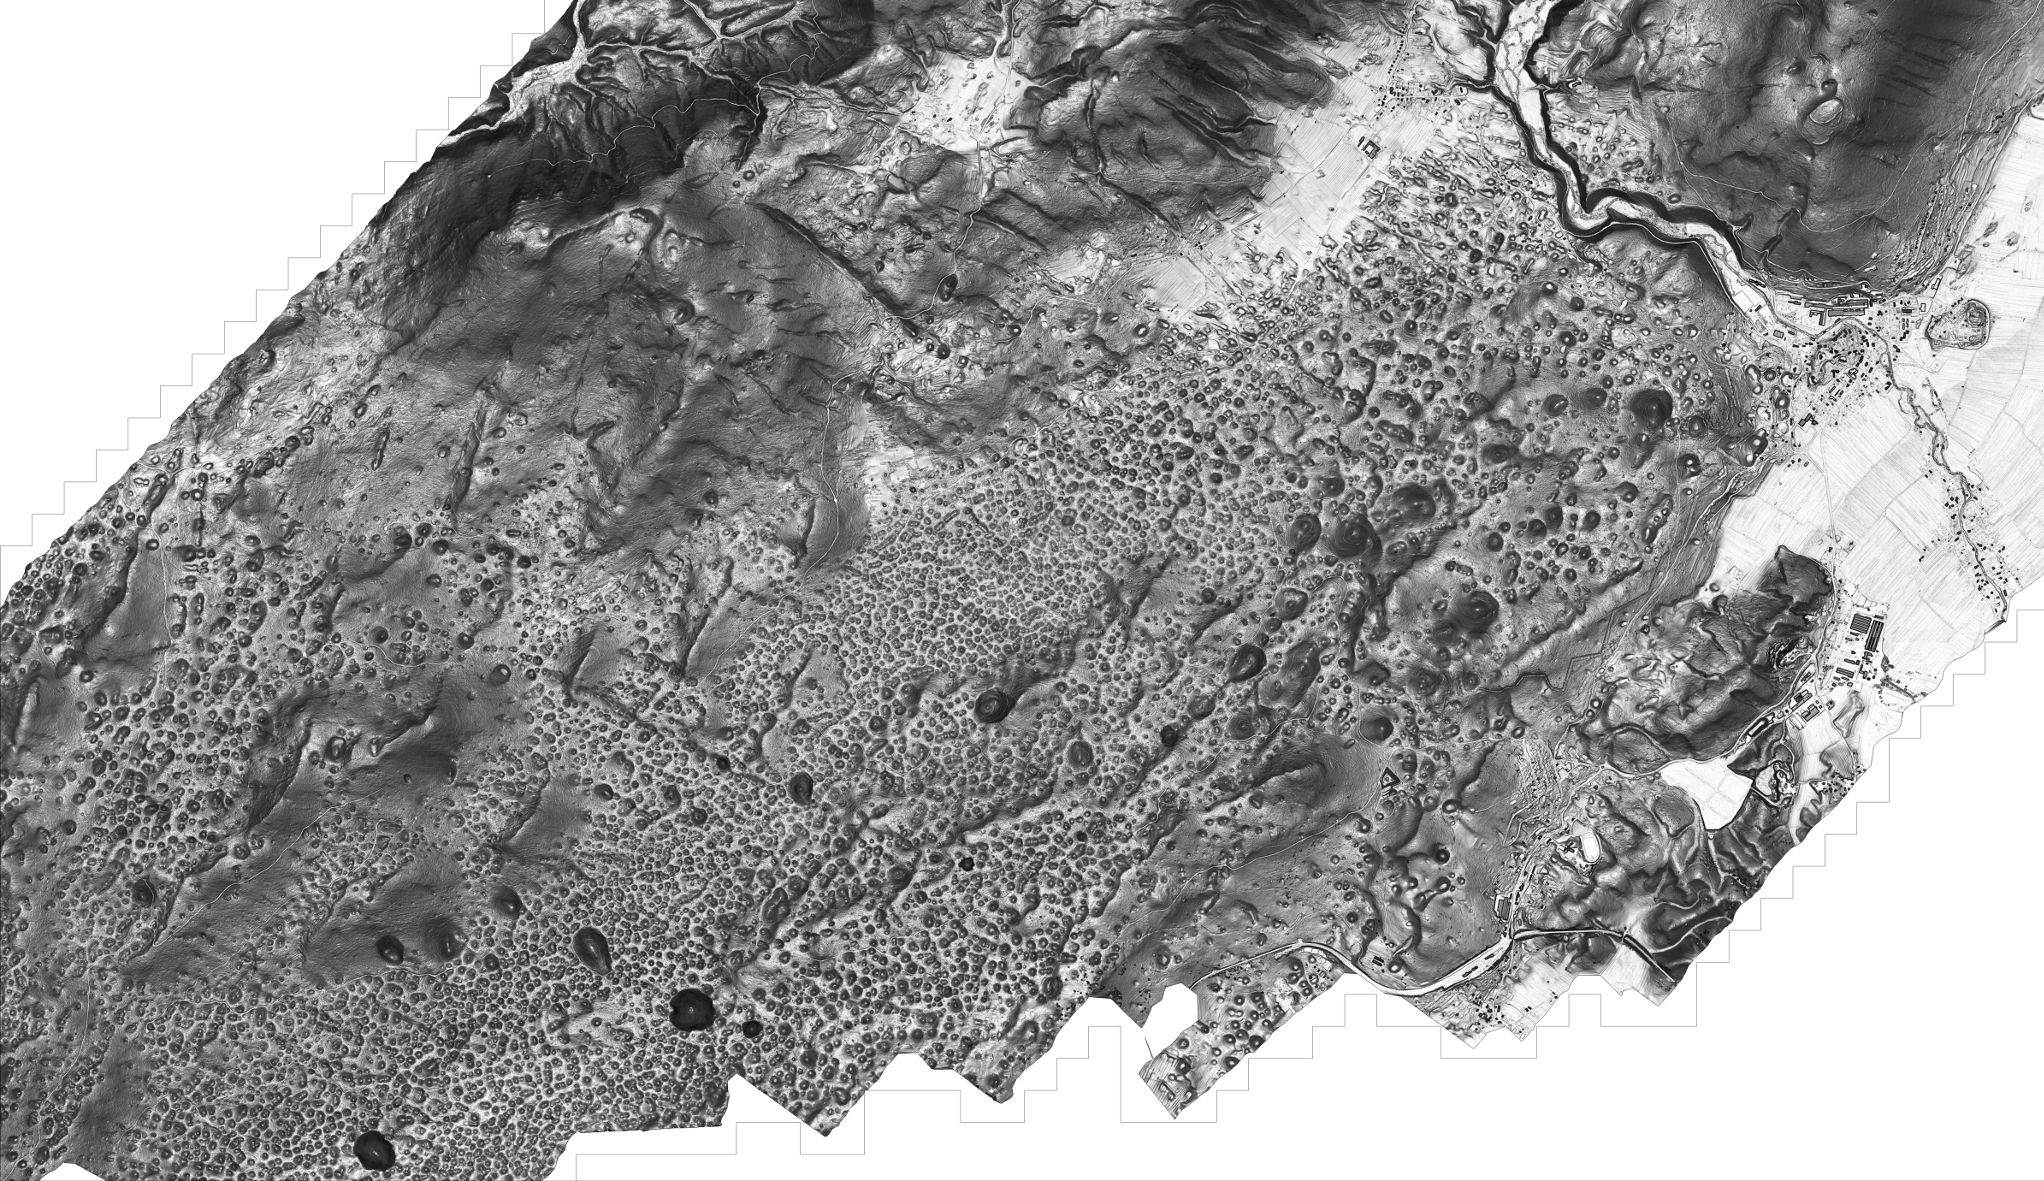
\includegraphics[width=14cm]{slike/menisija-relief.png}
  \caption{Menišija, $60 km^2$ območje med Cerknico in Logatcem vsebuje nekaj tisoč vrtač in več udornic}
  \label{fig:menisija-relief}
\end{figure}

\chapter{Preučevanje realnih vrtač}

Vrtače so zaobljene lijakaste globeli, globine nekaj metrov in premera nekaj deset metrov. Za identifikacijo velike količine vrtač se poslužimo računske metode, ki jo uporabljajo tudi drugi avtorji \cite{doctor13} - izračunamo indeks konkavnosti reliefa in na podlagi le-tega klasificiramo dele površja kot vrtače.

Konkavni objekti, ki jih najdemo imajo porazdelitev efektivnih polmerov (\mbox{$r_{eff}=\frac{\sqrt{A_{eff}}}{\pi}$}), kot vidno na sliki \ref{fig:menisija-polmeri-hist}.

\begin{figure}[H]
  \centering
  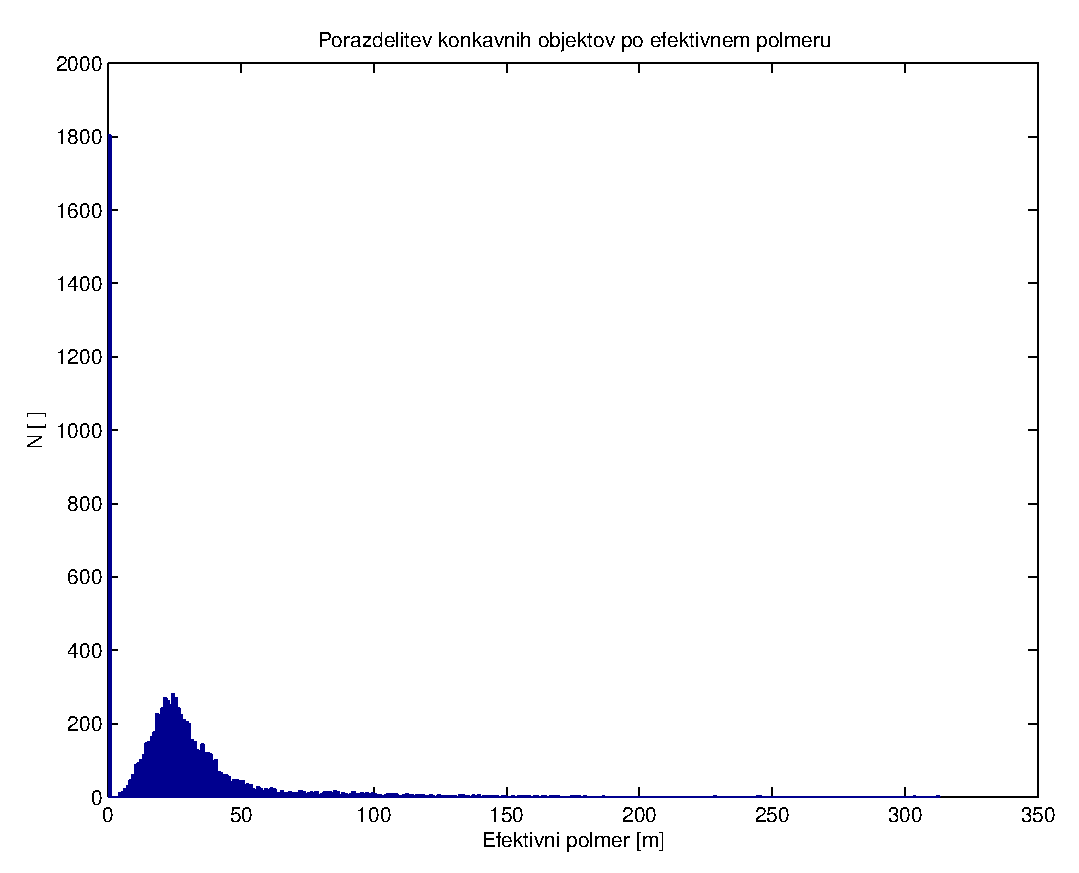
\includegraphics{slike/menisija-polmeri-hist}
  \caption{Polmeri konkavnih objektov v Menišiji, vrh pade v razred od 16m do 17m}
  \label{fig:menisija-polmeri-hist}
\end{figure}

Poradelitev efektivnih polmerov daje slutiti, da obstaja ravnovesna velikost vrtače, h kateri konvergirajo vse globeli v območju ne glede na njihov nastanek.
To nas napelje na misel, da obstaja tudi ravnovesna oblika vrtače, ki bi se pojavila na idelani podlagi, če bi preteklo dovolj časa.

Posamezne realne vrtače zaradi lokalnih pogojev niso simetrične, a zdi se da so si med seboj podobne. Da bi ugotovili idealno obliko vrtače izračunamo povprečje velikega števila realnih vrtač. Uporabimo dva pristopa - pri prvem (Slika \ref{fig:menisija-vrtaca}) vrtače različnih velikosti raztegnemo, pri drugem (Slika \ref{fig:menisija-vrtace-po-razredih}) pa jih razdelimo v velikostne razrede in jih povprečimo znotraj le-teh. 

\begin{figure}[H]
  \centering
  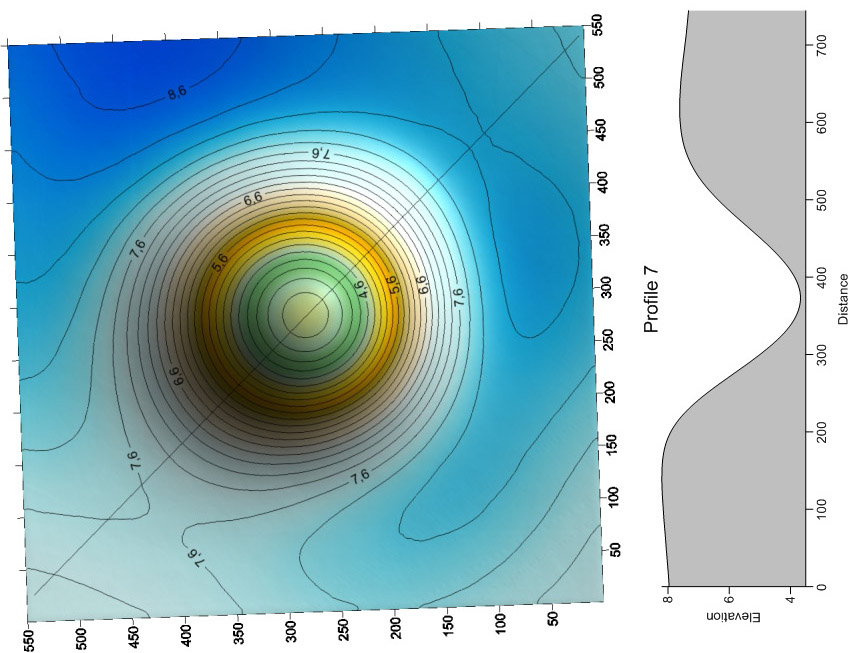
\includegraphics[width=7cm]{slike/vrtaca-menisija}
  \caption{Povprečje 8687 realnih vrtač z območja Menišije, pred povprečjem so bile vrtače raztegnjene na velikost največje v setu.}
  \label{fig:menisija-vrtaca}
\end{figure}

\begin{figure}[H]
  \centering
  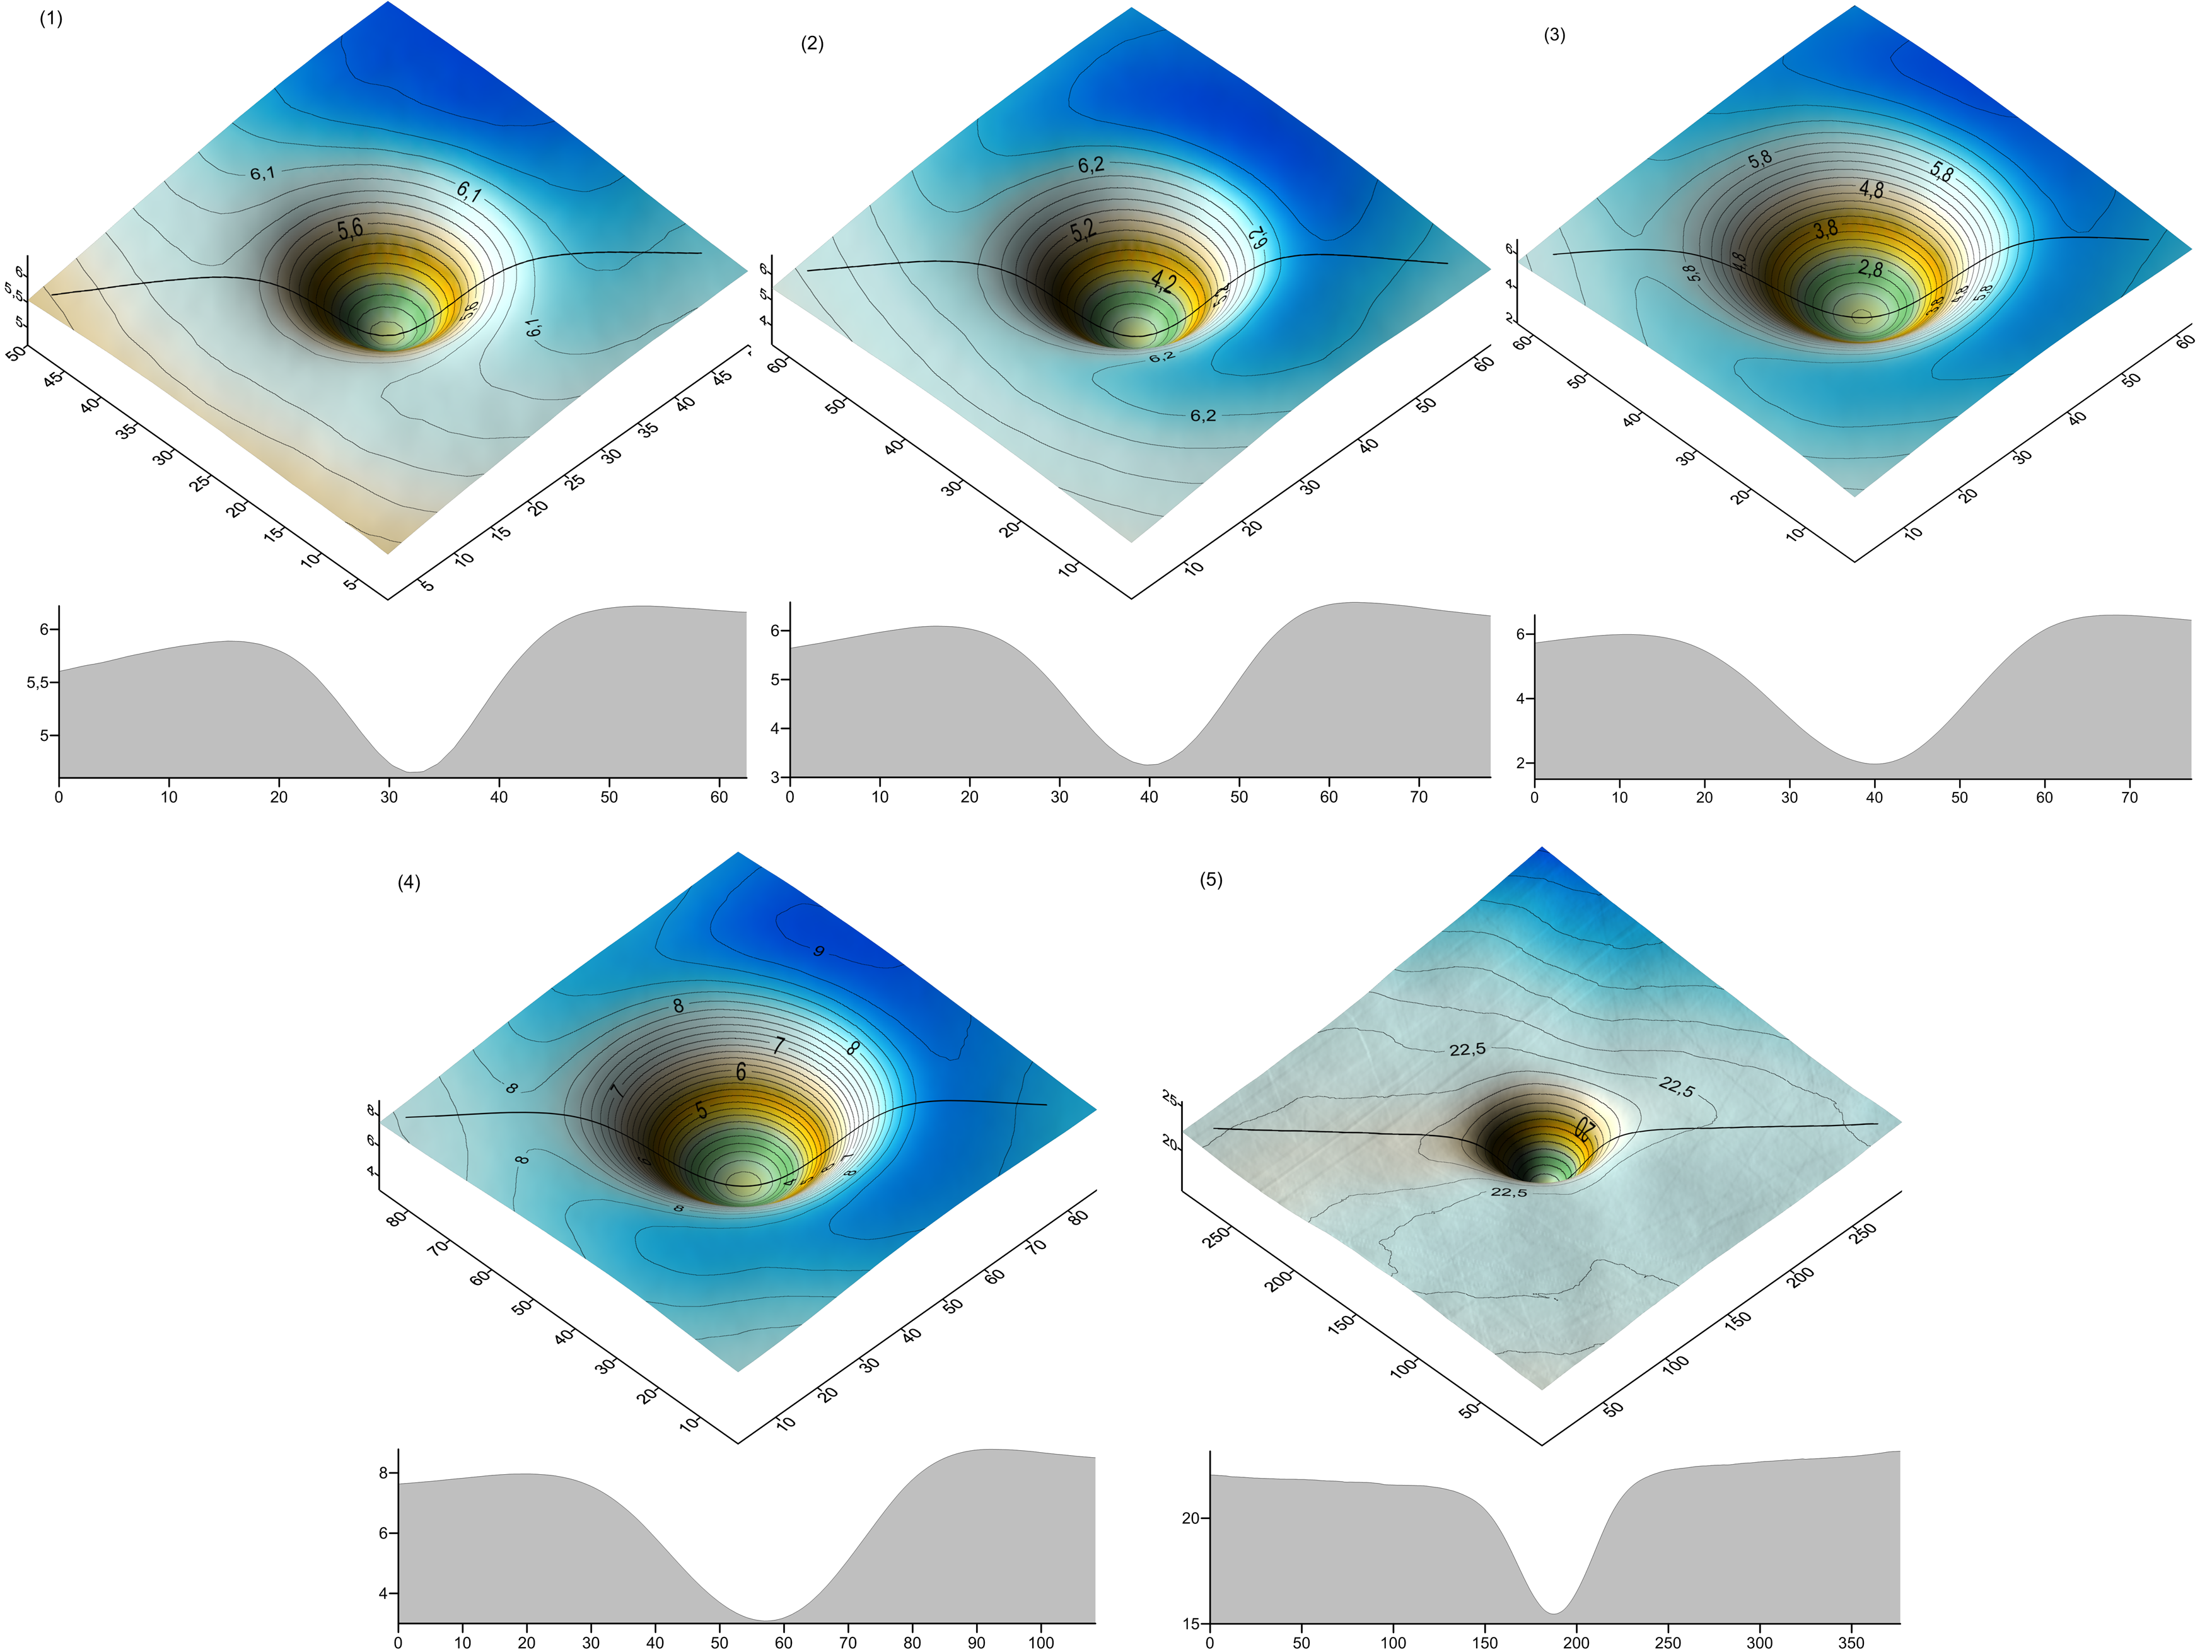
\includegraphics[width=13cm]{slike/vrtace-po-razredih-menisija}
  \caption{Vrtače po velikosti razdelimo v pet razredov (najmanjša petina gre v prvi razred, itn.), in jih znotraj razredov povprečimo.}
  \label{fig:menisija-vrtace-po-razredih}
 \end{figure}

Na prvi pogled se zdijo profili dobljenih oblik gaussove oblike (\ref{fit-vrtace}), kar ne zbuja nujno zaupanja v metodo. Prav tako se ne zdi, da bi bil ta rezultat pretirano fizikalno uporaben.

\begin{equation}
  f(x,y) = A \cdot e^{-\frac{(x-x_0)^2}{\sigma_x^2}-\frac{(y-y_0)^2}{\sigma_y^2}} + B \cdot x + C \cdot y + D  
  \label{fit-vrtace}
\end{equation}

Rezultat vseeno uporabimo tako da gaussovo funkcijo nalegamo na realne vrtače in tako dobimo precej dobre lokacije njihovih najnižjih točk, ter njihove $\sigma_x$ in $\sigma_y$. Z lokacijami najnižjih točk lahko izmerimo povprečne profile vrtač, ki imajo enake efektivne polmere, naprimer: Slika \ref{fig:menisija-profil-21}

\begin{figure}[H]
  \centering
  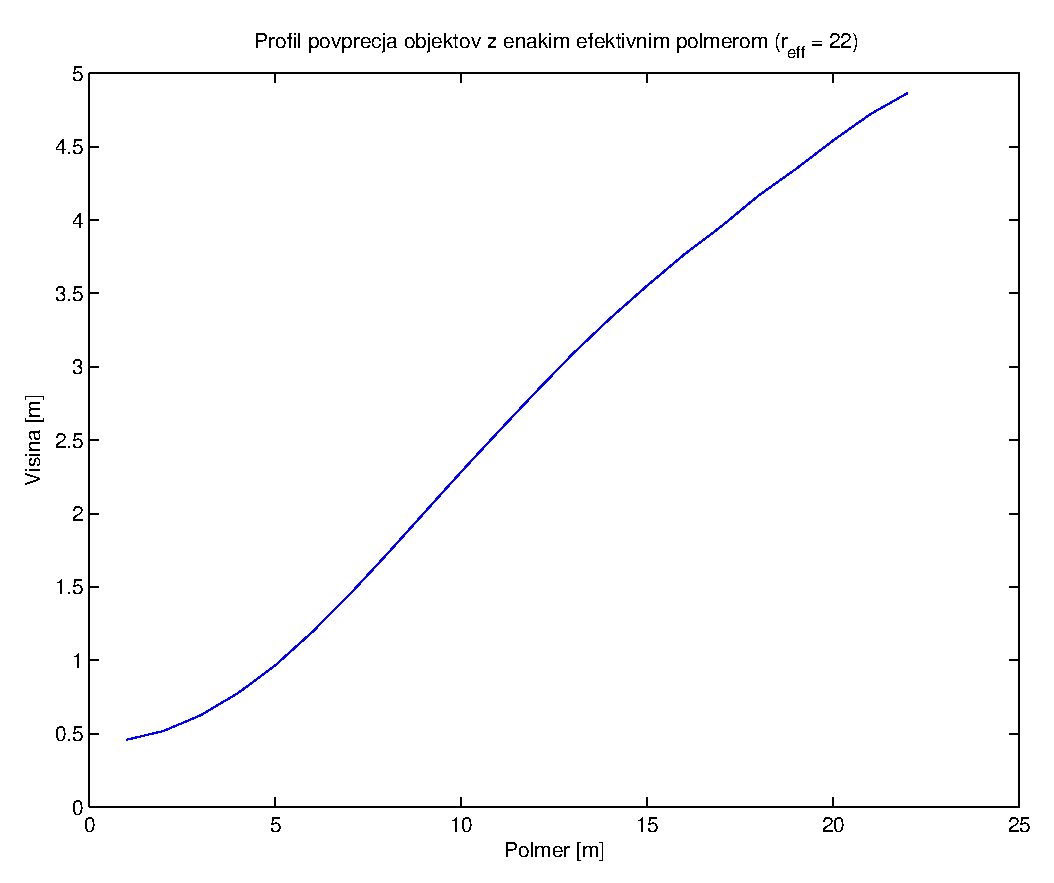
\includegraphics{slike/menisija-profil-21}
  \caption{Povprecje profilov vrtač z efektivnimi polmeri med 21,5m in 22,5m }
  \label{fig:menisija-profil-21}
\end{figure}

Če pa vse profile združimo v eno sliko, tako da polmer postavimo v smeri osi $y$ in efektivni polmer v smeri $x$ osi, dobimo sledečo sliko \ref{fig:menisija-profil-profilov}

\begin{figure}[H]
  \centering
  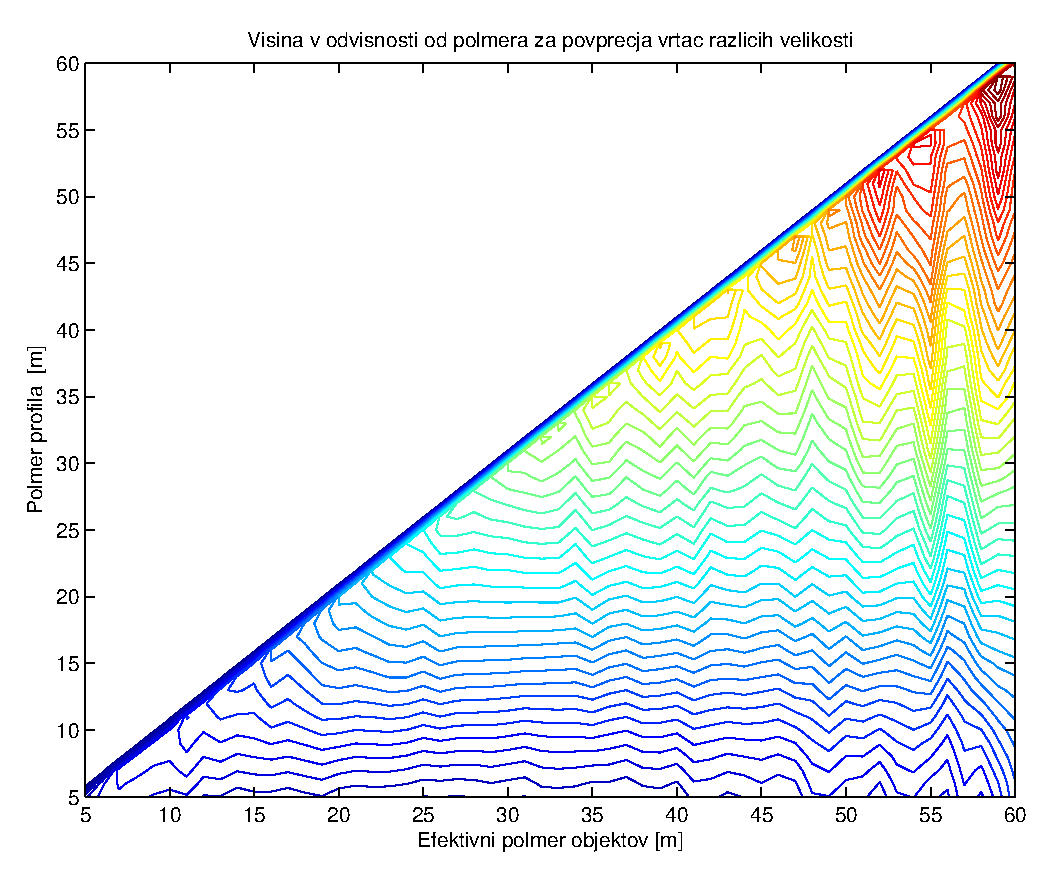
\includegraphics{slike/menisija-profil-profilov}
  \caption{Odvisnost profila vrtace od velikosti vrtace}
  \label{fig:menisija-profil-profilov}
\end{figure}

Zdi se torej, da so si vrtače podobne oblike ne glede na velikost in to po celi njihovi površini, le v normalno površje se iztečejo prej ali kasneje, a zopet na podoben način.
Če na dobljene profile ponovno nalegamo gaussovko (\ref{fit-profila}) vidimo, da to ne drži popolnoma.  

\begin{equation}
  f(x) = A \cdot e^{-\frac{(x-x_0)^2}{\sigma_x^2}} + C  
  \label{fit-profila}
\end{equation}


\chapter{Numerično modeliranje vrtač} 
\label{ch2}

\section{Model naključnih korozijskih toče}
\section{Naključne korozjske točke na realni kamnini}
\section{Preizkus modela korozijskih točk na geološki karti}


\chapter{Analitično modeliranje vrtač}
\label{ch3}

\section{Elastomehanični model}
\section{Boussinesqov približek}


%%%%%%%%%%%%%%%%%%%%%%%%%%%%%%%%%%%%%%%%
\begin{comment}
%%%%%%%%%%%%%%%%%%%%%%%%%%%%%%%%%%%%%%%%

\chapter{Zaključek}


%%%%%%%%%%%%%%%%%%%%%%%%%%%%%%%%%%%%%%%%
\end{comment}
%%%%%%%%%%%%%%%%%%%%%%%%%%%%%%%%%%%%%%%%

\nocite{*}
\newpage
\bibliography{bibliography}{}
\bibliographystyle{alpha}


\end{document}

